\label{ch:results}

\section{End-to-end serving results}

\Cref{tab:e2e-results} reports the clean A/B measurement. Both conditions
completed all 500 requests. Enabling batching shortened total benchmark
duration from \SI{4756.098}{s} to \SI{4650.166}{s}, a difference of
\SI{105.932}{s}. Output throughput increased from 31.54 to 32.26 tokens/s, or
2.28\%.

\begin{table}[p]
  \centering
  \caption{End-to-end serving results. Lower is better for all latency
  columns; higher is better for throughput. Each condition is one run.}
  \label{tab:e2e-results}
  \resizebox{\textwidth}{!}{%
  \begin{tabular}{lrrrrrrr}
    \toprule
    Batching & Duration (s) & Output tok/s &
    TTFT P50 & TTFT P99 & TPOT P50 & TPOT P99 & E2E P50 / P99 \\
    \midrule
    Off & 4756.10 & 31.54 & 49180.71 & 75740.25 & 828.53 & 1007.82 & 303462.69 / 322184.88 \\
    On  & 4650.17 & 32.26 & 48599.04 & 74756.17 & 812.44 & 999.01 & 293821.76 / 317351.61 \\
    \bottomrule
  \end{tabular}}
  \vspace{1mm}

  \footnotesize Latency values are milliseconds.
\end{table}

All six reported latency percentiles moved in the favorable direction.
Median/P99 TTFT decreased by 1.18\%/1.30\%; median/P99 TPOT decreased by
1.94\%/0.87\%; and median/P99 E2E latency decreased by 3.18\%/1.50\%.
The larger improvement in median E2E than in an individual TTFT or TPOT
percentile should not be interpreted as an algebraic sum of percentile changes:
each percentile may correspond to a different request, and E2E accumulates
many decode intervals.

\begin{figure}[t]
  \centering
  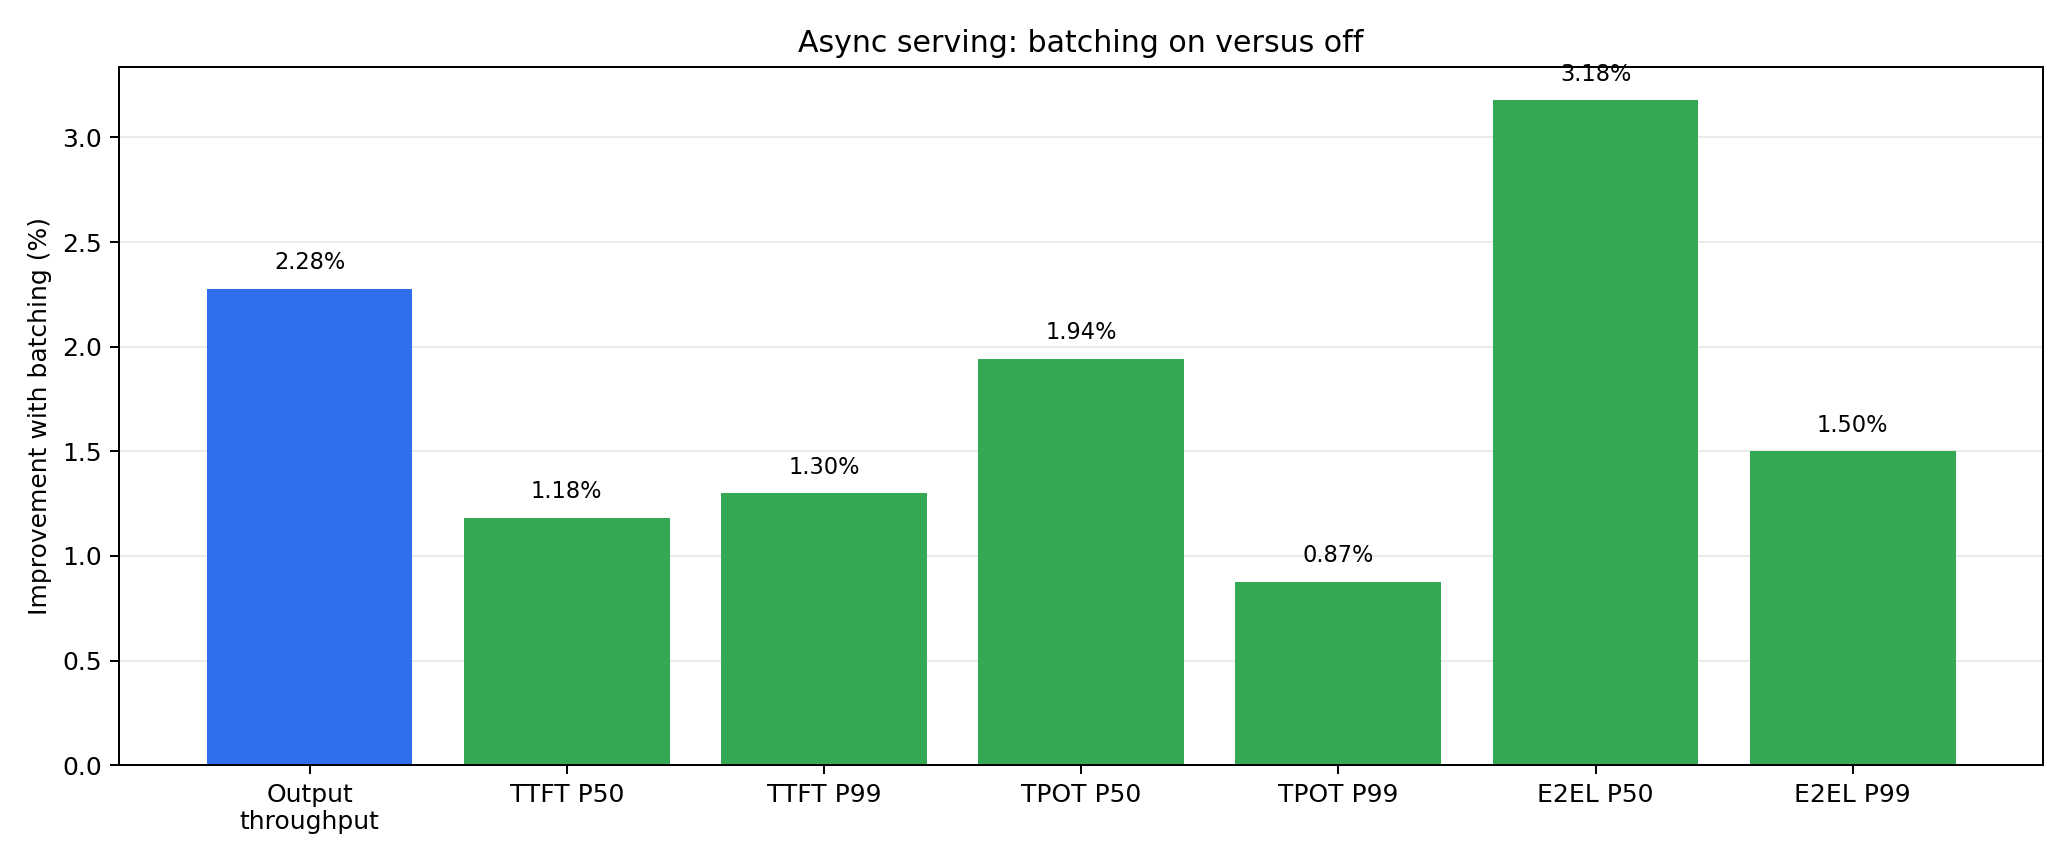
\includegraphics[width=0.92\textwidth]{e2e_improvement.png}
  \caption{Relative improvement with batching enabled in the clean A/B run.
  Positive values indicate higher throughput or lower latency.}
  \label{fig:e2e-improvement}
\end{figure}

The direction is consistent with the hypothesis that migration bursts interfere
with inference. TTFT improves despite batching being a background migration
optimization because the benchmark mixes prefill and decode across concurrent
requests. TPOT improves because decode continues throughout asynchronous
migration. The result does not isolate which inference communication operation
benefited; it measures the user-visible aggregate effect.

\section{Network traffic}

The head-node P99 of aggregate RX+TX traffic decreased from 599.81 MB/s to
538.40 MB/s, a reduction of 10.24\%. This is the largest relative change among
the reported measurements and directly concerns the mechanism targeted by the
scheduler: smoothing extreme network demand rather than reducing total expert
bytes.

\begin{figure}[p]
  \centering
  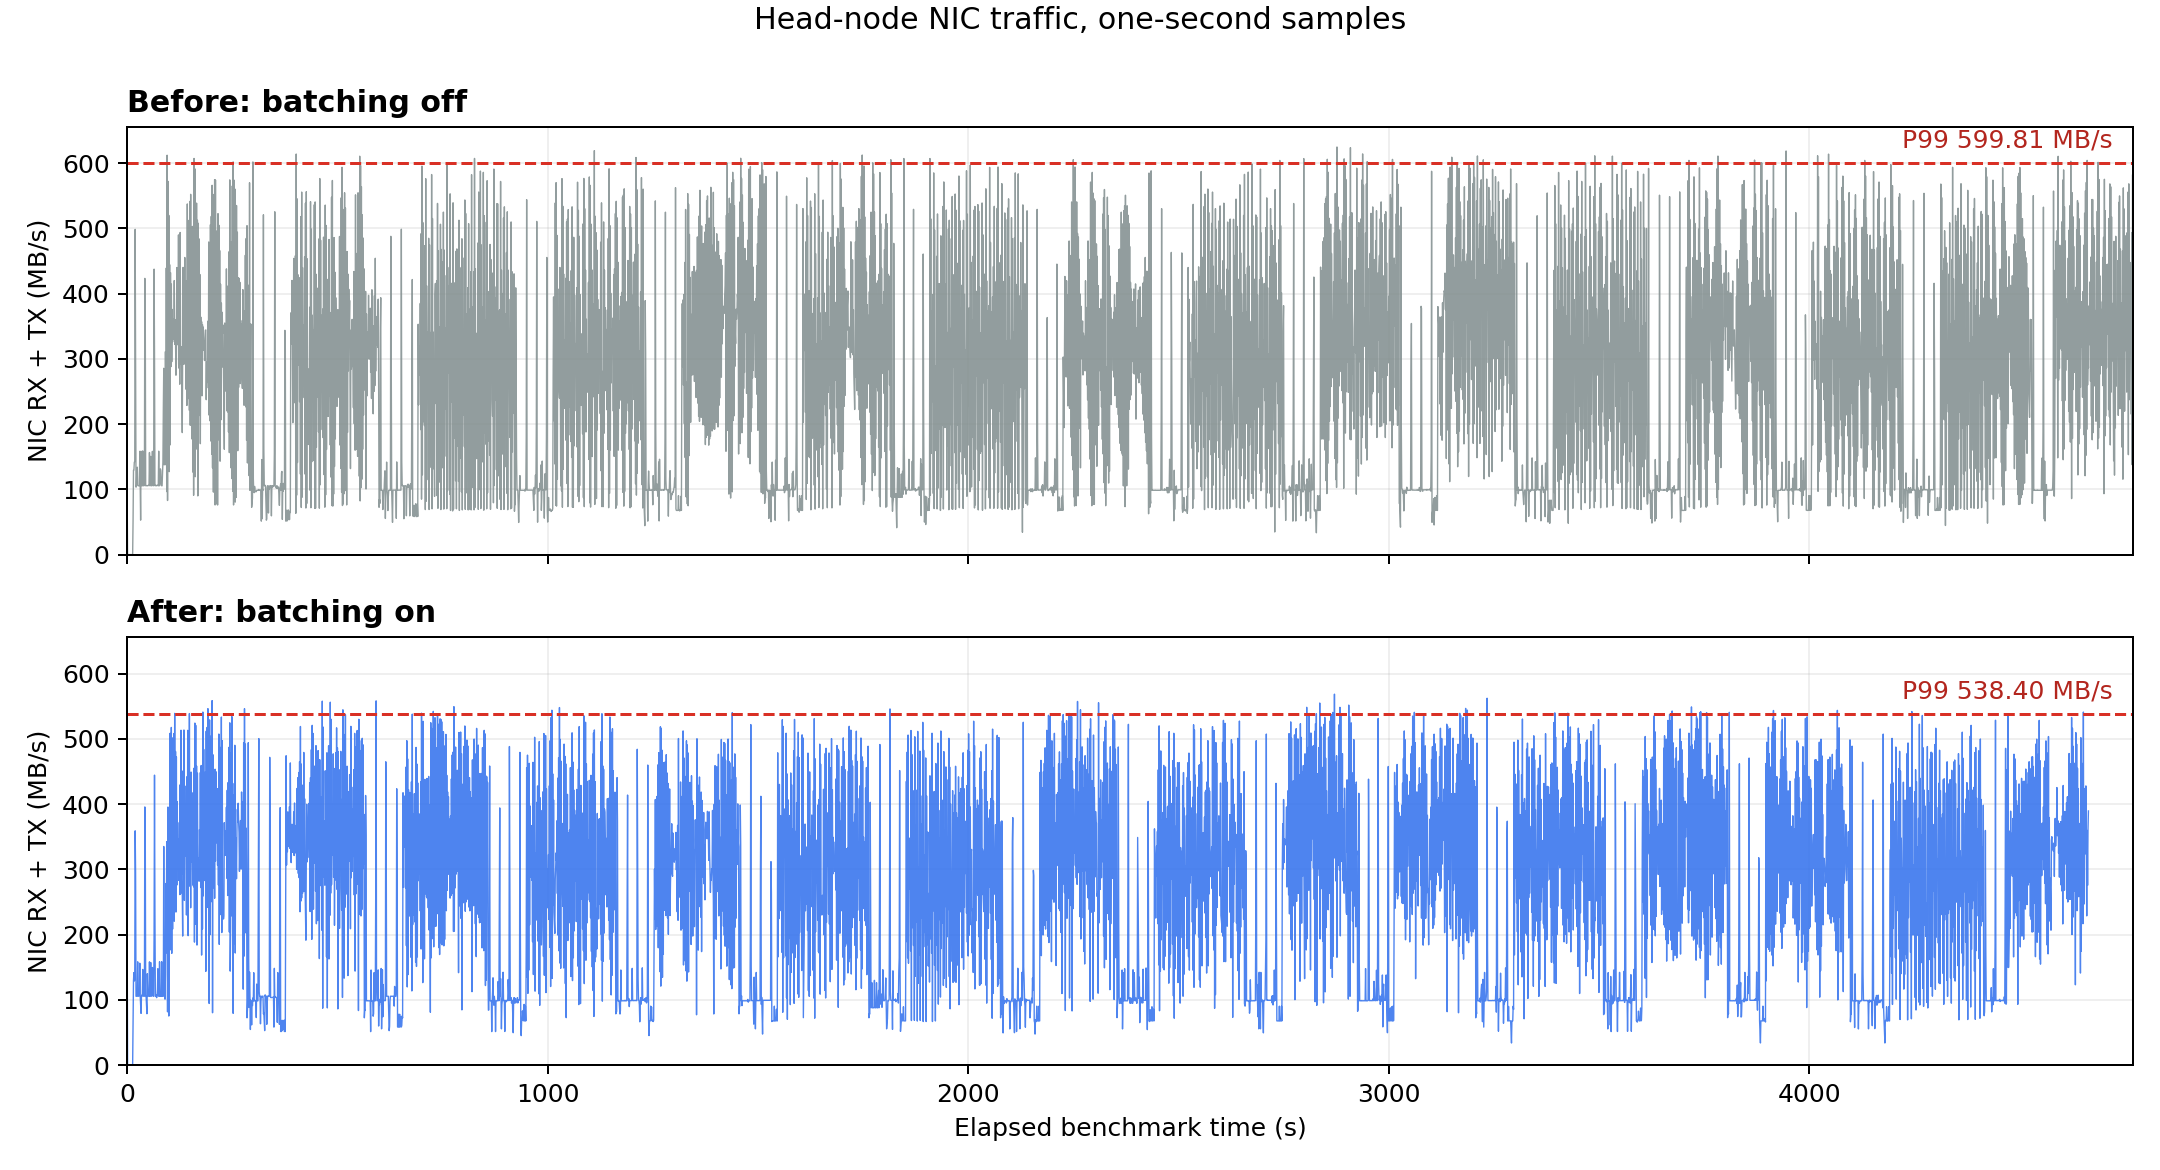
\includegraphics[width=\textwidth]{nic_timeseries.png}
  \caption{Head-node aggregate NIC traffic sampled once per second during the
  two independent runs. Batching reduces the high tail of observed traffic.}
  \label{fig:nic-series}
\end{figure}

\Cref{fig:nic-series} shows that traffic is bursty in both configurations.
This is expected: inference itself communicates and EPLB continues to migrate
whole expert tensors. The scheduler does not impose a byte-rate limiter. It
limits per-rank flow concurrency, spreading conflicting migration flows across rounds.
The lower P99 supports the contention explanation, but the two time series are
not temporally aligned executions of identical low-level events. They are
separate A/B runs with the same client workload.

The measurement also has a scope limitation. Only the head node was sampled,
so the result does not prove that every worker's P99 decreased. Because the
scheduler enforces the same rank-degree constraint globally, lower bursts are
plausible on other ranks, but per-node counters are necessary to verify that
claim.

\section{Scheduler profiling}
\label{sec:profile-results}

All four ranks recorded 34 calls to the cycle-wide scheduling range during the
formal profiling window. Since one call prepares all 48 layer schedules, the
trace represents 34 rebalance-cycle scheduling events per rank, not
$34\times48$ independent top-level calls.

\begin{table}[t]
  \centering
  \caption{NVTX elapsed time for cycle-wide scheduler calls.}
  \label{tab:profile}
  \begin{tabular}{rrrrr}
    \toprule
    Rank & Calls & P50/call (ms) & P99/call (ms) & Cumulative (ms) \\
    \midrule
    0 & 34 & 7.819 & 17.536 & 302.081 \\
    1 & 34 & 7.090 & 12.357 & 253.152 \\
    2 & 34 & 7.035 & 16.104 & 255.239 \\
    3 & 34 & 7.005 & 8.103  & 241.190 \\
    \bottomrule
  \end{tabular}
\end{table}

Median elapsed time is between 7.01 and 7.82 ms per rank per rebalance cycle.
Dividing by 48 gives roughly 0.146--0.163 ms per layer as an intuition, but the
implementation and profiler measure one aggregated call, so this quotient is
not presented as an independently observed per-layer latency. P99 variability
is larger, consistent with host scheduling and interference in the background
thread.

Rank 0 has the largest cumulative cost, \SI{302.081}{ms}. Ranks execute on
separate hosts and schedule concurrently, so adding the four cumulative values
would overstate wall-clock overhead. Applying \cref{eq:cost-ratio} to the clean
A/B saving gives

\begin{equation}
  R=\frac{0.302081}{4756.098161-4650.165779}\times100\%
   =0.285\%.
\end{equation}

\begin{figure}[t]
  \centering
  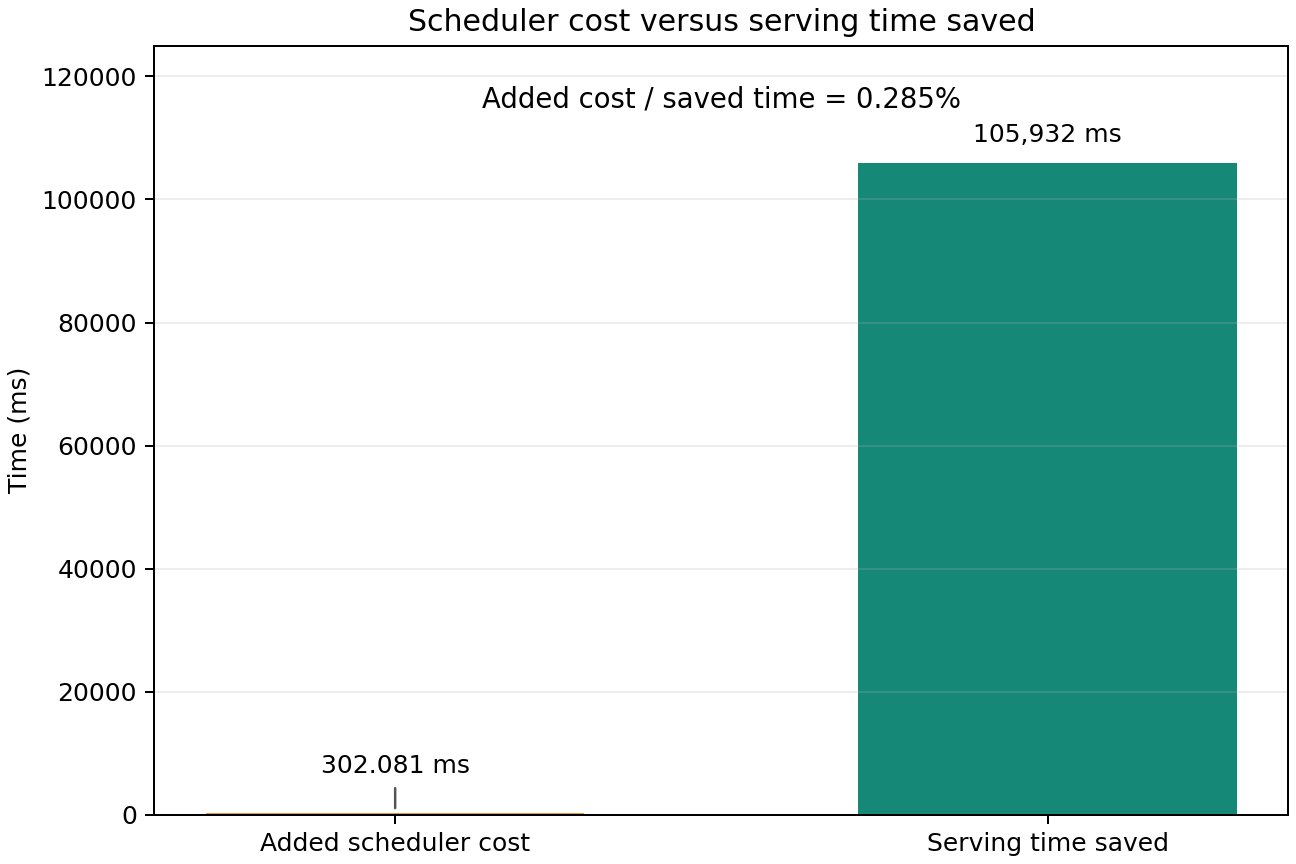
\includegraphics[width=0.82\textwidth]{scheduler_cost_vs_saved.png}
  \caption{Largest measured cumulative scheduler time versus serving time
  saved. The linear axis intentionally preserves the scale difference.}
  \label{fig:cost-saved}
\end{figure}

This comparison shows that the measured scheduler cost is small relative to
the observed completion-time difference. It is not a causal decomposition of
the saving: the profiler run is separate, and the 105.932 s difference includes
all downstream effects. It nevertheless answers the maintainer-facing systems
question of whether the additional Python scheduling work is of the same order
as the apparent benefit. It is not.

\section{Answering the research questions}

\paragraph{RQ1: representation.}
The directed migration-flow graph captures endpoint contention cleanly, while
the topology-aware ILP adds routed-link capacity for offline reasoning. The ILP
example confirms that minimizing foreground contention can intentionally
increase migration completion time.

\paragraph{RQ2: online scheduling.}
Coalescing by directed rank pair followed by first-fit edge coloring provides a
deterministic and dependency-free rule. The bit-mask representation makes the
central constraint explicit and inexpensive. It is not guaranteed to minimize
batch count, but exact color optimality is not required for safe throttling.

\paragraph{RQ3: semantic integration.}
Tests show completeness, conflict freedom, local-copy exclusion, replica
balancing, deterministic output, and correct mock-communicator execution. The
implementation restores NIXL context and executes each batch separately,
precomputes all layer schedules once per cycle, and leaves synchronous and
disabled paths unchanged.

\paragraph{RQ4: serving impact.}
In the evaluated cluster, every reported throughput or latency metric improved,
and NIC P99 decreased by 10.24\%. Scheduler profiling found a conservative
cost-to-saved ratio of 0.285\%. These results are consistent with reduced
migration interference and justify the implementation for this environment.

\section{Discussion}

The results illustrate why migration duration alone is the wrong optimization
target for asynchronous EPLB. A scheduler can add communication rounds yet
improve total serving completion time, because the foreground model continues
to execute during those rounds. The relevant resource is not only bytes moved
but how aggressively those bytes are injected while latency-sensitive traffic
is active.

The rank-disjoint-flow constraint is deliberately conservative. On $n$ ranks,
at most $\lfloor n/2\rfloor$ independent directed flows appear in a batch. A
topology-aware scheduler might safely allow greater rank participation when
ranks are co-located, use separate NICs, or have available bandwidth. The
fixed rule trades peak migration speed for predictable behavior and
portability without topology discovery.

Cycle-wide precomputation addresses a different concern: CPU overhead. It does
not make network batches coarser and does not transfer 48 layers together. It
reduces top-level scheduling invocations while preserving layer-wise migration.
This separation between scheduling granularity and transfer granularity is a
key engineering result of the work.

\section{Threats to validity}

\subsection{Internal validity}

The off run preceded the on run, so temporal drift, thermal state, background
load, or network state may contribute to the difference. Fresh servers and an
identical warm-up reduce but do not eliminate these effects. Only one run per
condition was retained; repeated interleaved runs would provide stronger
evidence. The client uses the same seed, yet stochastic system scheduling means
request timing is not identical.

NIC counters include all interface traffic. They cannot distinguish NIXL
migration bytes from Ray control traffic, model communication, or unrelated
traffic. A packet or transport-level trace and counters on every node would
strengthen causal attribution. Still, the lower NIC P99 and favorable serving
metrics are mutually consistent.

\subsection{Construct validity}

The ILP slowdown equation is a deliberately linear surrogate. Queueing and
protocol effects are nonlinear, and flow weights count experts rather than
bytes or measured transfer time. The ILP result should therefore be read as a
design demonstration. The E2E benchmark, not the ILP objective value, is the
evidence for real serving behavior.

The random-token workload fixes lengths and activates frequent EPLB, but it is
not a production request distribution. Ignoring EOS makes output work
deterministic but removes natural variation. Prefix caching is enabled, which
improves realism relative to disabling it, although random prefixes offer
limited sharing.

\subsection{External validity}

The cluster has four older GPUs and \SI{10}{Gb/s} Ethernet without RDMA.
Production systems may use NVLink within nodes and 100--400 Gb/s RDMA between
nodes. Higher bandwidth can reduce contention, whereas larger models and more
ranks can increase the number and size of migrations. Results may therefore be
smaller or larger in another environment.

Only Qwen3-30B-A3B-Instruct-2507 and NIXL 1.3.2 were used in the final study.
The code supports the vLLM communicator abstraction, but backend-specific
progress and synchronization behavior can change batch overlap. Separate
evaluation is needed for Gloo and future NIXL versions.

\subsection{Conclusion validity}

The results are effect estimates from a single A/B pair, not confidence
intervals. The thesis consequently avoids terms such as ``statistically
significant'' and does not generalize the exact percentages. The strongest
supported conclusion is conditional: under this documented configuration,
batching coincided with lower NIC tail traffic and improvements in all reported
serving metrics at a small measured scheduling cost.
